\documentclass{sig-alternate}

% Packages.tex

% Packages di latex utilizzati 

  % Standard dell'ams
\usepackage{amssymb,amsmath}

  % Per le definizioni di connessioni di Galois
\usepackage{galois}

  % Per formattare ed includere il testo
\usepackage{lgrind}
     % Cambiamento dei font per lgrind: tutti in Courier
\def\CMfont{\ttfamily\itshape}
\def\KWfont{\ttfamily\bfseries}
\def\VRfont{\ttfamily}
\def\BGfont{\ttfamily}
\def\NOfont{\ttfamily}

  % Caratteri speciali per i nomi di funzione
\usepackage{bbm}

  % Caratteri ``cal'' carini
\usepackage[mathcal]{euscript}

  % per \baro
\usepackage{stmaryrd}

  % per \xspace
\usepackage{xspace}

  % per i diagrammi
\usepackage[all]{xy}

  % for scalebox
\usepackage{graphicx}
 
   % Per le figure incastrate l'una nell'altra
\usepackage{subfigure}

  % Per le figure nel testo
\usepackage{wrapfig}


\usepackage{tabularx}

  % Per includere i verbatim
\newbox\subfigbox
\makeatletter
\newenvironment{subfloat}
{\def\caption##1{\gdef\subcapsave{\relax##1}}%
\let\subcapsave\@empty
\setbox\subfigbox\hbox
\bgroup}
{\egroup
\subfigure[\subcapsave]{\box\subfigbox}}
\makeatother

   % Per la compilazione Condizionale
\usepackage{ifthen}

\usepackage{empheq}

   % Per i riferimenti incrociati



%\ifx\pdfoutput\undefined % Se compilo con ``latex'' ed uso ps2pdf
%\usepackage{color}
%\usepackage[dvips]{graphicx}       %%% graphics for dvips
%\DeclareGraphicsExtensions{.eps}   %%% standard extension for included graphics
%\usepackage[bookmarks=true]{hyperref}
%\else                    % Se compilo con ``pdflatex'' 
%\usepackage[pdftex]{graphicx}      %%% graphics for pdfLaTeX 
%\DeclareGraphicsExtensions{.pdf}   %%% standard extension for included graphics
%\usepackage[pdftex]{thumbpdf}      %%% thumbnails for pdflatex
%\usepackage[pdftex,                %%% hyper-references for pdflatex
%bookmarks=true,%                   %%% generate bookmarks ...
%bookmarksnumbered=true,%           %%% ... with numbers
%hypertexnames=false,%              %%% needed for correct links to figures !!!
%breaklinks=true,%                  %%% break links if exceeding a single line
%linkbordercolor={0 0 1}]{hyperref} %%% blue frames around links
%                                  %%% pdfborder={0 0 1} is the default
%\hypersetup{
%pdfauthor   = {Francesco Logozzo \& Agostino Cortesi},
%pdftitle    = {to be decided},
%pdfsubject  = {Objects},
%pdfkeywords = {Abstract Interpretation, Static Analysis, Object Oriented}
%}
%\pdfadjustspacing=1                %%% force LaTeX-like character spacing
%\fi 


%%% Local Variables: 
%%% mode: plain-tex
%%% TeX-master: "main"
%%% End: 

% Definizione dei simboli

\newcommand{\eg}{\textit{e.g.}}
\newcommand{\ie}{\textit{i.e.}}

% Definizione dell' operatore di astrazione
\newcommand{\abs}[1]{\ensuremath{\bar{\mathsf{#1}}}}

\newcommand{\sx}{\llbracket}
\newcommand{\dx}{\rrbracket}

  % Semantica generica
\newcommand{\sem}[1]{\ensuremath{\sx \mathtt{#1} \dx}}

  % Semantica che prende un nome
\newcommand{\semantica}[2]{\ensuremath{\mathbb{#1}\sem{#2}}}

\newcommand{\BigSemantica}[2]{\ensuremath{\mathbb{#1}{\Bigg\llbracket #2 \Bigg\rrbracket}}}

  % Semantiche generiche
\newcommand{\csem}[1]{\ensuremath{\semantica{s}{#1}}}
\newcommand{\asem}[1]{\ensuremath{\semantica{\abs{s}}{#1}}}
\newcommand{\asemRefined}[1]{\ensuremath{\semantica{\abs{s}^*}{#1}}}

  % Funzione di ``transfer''
\newcommand{\trasf}[1]{\ensuremath{\semantica{t}{#1}}}
\newcommand{\atrasf}[1]{\ensuremath{\semantica{\abs{t}}{#1}}}

  % Semantica di: costruttore,  metodo
\newcommand{\semcostr}[1]{\semantica{i}{#1}}
\newcommand{\semmetodo}[1]{\semantica{m}{#1}}
\newcommand{\semoggetto}[1]{\semantica{o}{#1}}
\newcommand{\semclasse}[1]{\semantica{c}{#1}}

  % Semantica Colleting Traces
\newcommand{\Semmetodo}[1]{\semantica{M}{#1}}
\newcommand{\Semoggetto}[1]{\semantica{O}{#1}}
\newcommand{\Semclasse}[1]{\semantica{C}{#1}}

  % Semantics Reachable States
\newcommand{\rsemcostr}[1]{\semantica{I}{#1}}
\newcommand{\rsemmetodo}[1]{\Semmetodo{#1}}
\newcommand{\rsemoggetto}[1]{\semantica{O}{#1}}
\newcommand{\rsemclasse}[1]{\semantica{C}{#1}}

  % Seamntica Astratta
\newcommand{\asemcostr}[1]{\semantica{\bar{I}}{#1}}
\newcommand{\asemmetodo}[1]{\semantica{\bar{M}}{#1}}
\newcommand{\asemoggetto}[1]{\semantica{\bar{O}}{#1}}
\newcommand{\asemclasse}[1]{\semantica{\bar{C}}{#1}}

  % Operazioni su stati
\newcommand{\less}{\ensuremath{\sqsubseteq}}
\newcommand{\join}{\ensuremath{\sqcup}}
\newcommand{\meet}{\ensuremath{\sqcap}}
\newcommand{\bottom}{\ensuremath{\bot}}
\newcommand{\bigjoin}{\ensuremath{\bigsqcup}}

  % Semantica astratta
\newcommand{\asemantica}[2]{\semantica{\bar{#1}}{#2}}
\newcommand{\asemanticaBig}[2]{\BigSemantica{\bar{#1}}{#2}}


  % Semantica astratta BIS, per aggiungere pedici
\newcommand{\asemanticaBis}[3]{\semantica{\bar{#1}_{\textit{#2}}}{#3}}

  % Operazioni astratte
\newcommand{\nabs}[1]{\bar{#1}}
\newcommand{\abot}{\nabs{\bot}}
\newcommand{\atp}{\nabs{\ensuremath{\top}}}
\newcommand{\aless}{\nabs{\less}}
\newcommand{\asup}{\ensuremath{\nabs{\sqsupseteq}}}
\newcommand{\acup}{\ensuremath{\nabs{\sqcup}}}
\newcommand{\ajoin}{\acup}
\newcommand{\abigcup}[1]{\nabs{\bigsqcup_{#1}}}
\newcommand{\abigjoin}[1]{\abigcup{#1}}
\newcommand{\acap}{\ensuremath{\nabs{\sqcap}}}
\newcommand{\ameet}{\acap}
\newcommand{\abigcap}[1]{\nabs{\bigsqcap_{#1}}}
\newcommand{\abigmeet}[1]{\abigcap{#1}}


 % lfp : least fixpoint
\newcommand{\lfp}[2]{\ensuremath{\mathrm{lfp}^{#1}_{#2}}}

 % gfp: greatest fixpoint
\newcommand{\gfp}[2]{\ensuremath{\mathrm{gfp}^{#1}_{#2}}}


% Insiemi e Funzioni

  % Insieme, elemento di insieme, nessun elemento
\newcommand{\insieme}[1]{\ensuremath{\mathsf{#1}}}
\newcommand{\el}[1]{\ensuremath{\mathsf{#1}}}
\newcommand{\noel}{\el{\bot}}

  % Insieme delle parti
\newcommand{\parti}[1]{\ensuremath{\mathcal{P}{(#1)}}}
\newcommand{\partiFin}[1]{\ensuremath{\mathcal{P}_{\mathrm{fin}}{(#1)}}}


  % Elementi di insiemi
\newcommand{\noval}{\ensuremath{\baro}}

  % Cardinalita di inisiemi
\newcommand{\cardinalita}[1]{\ensuremath{\# #1}}

  % Env, Store, Addr, Val, Label : Scorciatoie
\newcommand{\env}{\insieme{Env}}
\newcommand{\Env}{\env}

\newcommand{\aenv}{\ensuremath{\bar{\env}}}

\newcommand{\store}{\insieme{Store}}
\newcommand{\Store}{\store}

\newcommand{\astore}{\ensuremath{\overline{\store}}}

\newcommand{\AState}{\abs{\Sigma}}
\newcommand{\astate}{\AState}

\newcommand{\addr}{\insieme{Addr}}
\newcommand{\Addr}{\addr}

\newcommand{\aaddr}{\ensuremath{\overline{\addr}}}

\newcommand{\Reference}{\insieme{Ref}}
\newcommand{\reference}{\reference}

\newcommand{\AReference}{\ensuremath{\overline{\Reference}}}

\newcommand{\val}{\insieme{Val}}

\newcommand{\etichetta}{\insieme{Label}}
\newcommand{\cont}{\ensuremath{\kappa}}

  % Stati
\newcommand{\stati}[1]{\ensuremath{\Sigma}}
  % Tracce
\newcommand{\tracce}[1]{\ensuremath{\mathcal{T}(#1)}}
  % Transizione
\newcommand{\tr}[1]{\ensuremath{\xrightarrow{#1}}}

  % Insieme di funzioni
\newcommand{\funzione}[2]{\ensuremath{[#1 \rightarrow#2]}}

  % Funzione vuota
\newcommand{\emptyfun}{\ensuremath{[\cdot]}}

  % Insieme di funzioni monotone e joim-morphism
\newcommand{\funmon}[2]{\ensuremath{[#1 \stackrel{m}{\longrightarrow} #2]}}
\newcommand{\funjoin}[2]{\ensuremath{[#1 \stackrel{\sqcap}{\longrightarrow} #2]}}

% Astratto
  % Dominio concreto
\newcommand{\dom}[1]{\insieme{#1}}

  % Dominio astratto
\newcommand{\adom}[1]{\ensuremath{{\mathsf{#1}}}}

 % Vari domini
\newcommand{\Intervals}{\dom{Intv}}
\newcommand{\LT}{\dom{LT}}
\newcommand{\Boxes}{\dom{Boxes}}
\newcommand{\DBM}{\dom{DBM}}
\newcommand{\Octagons}{\dom{Oct}}
\newcommand{\Polyhedra}{\dom{Poly}}
\newcommand{\Poly}{\Polyhedra}
\newcommand{\Lineq}{\dom{LinEq}}
\newcommand{\LinEq}{\Lineq}
\newcommand{\Karr}{\Lineq}
\newcommand{\Symbolic}{\dom{Symb}}
\newcommand{\Pentagons}{\dom{Pnt}}
\newcommand{\SubPolyhedra}{\dom{SubPoly}}
\newcommand{\SubPoly}{\SubPolyhedra}
\newcommand{\Subpoly}{\SubPolyhedra}

  % Elemento di dominio astratto
\newcommand{\ael}[1]{\ensuremath{\abs{\el{#1}}}}
\newcommand{\aelBis}[2]{\ensuremath{\abs{\el{#1}}_\el{#2}}}

  % Funzione di astrazione e concretizzazione
\newcommand{\alfa}{\ensuremath{\alpha}}
%\renewcommand{\gamma}{\ensuremath{\gamma}}
\newcommand{\gm}{\ensuremath{\gamma}}


% Funzioni usate nella tesi
  % Transizione basica
\newcommand{\prossimo}{\ensuremath{\mathrm{next}}}
%\newcommand{\next}{\ensuremath{\mathrm{next}}}
\newcommand{\nextDir}{\ensuremath{\mathrm{next_{dir}}}}
\newcommand{\nextInd}{\ensuremath{\mathrm{next_{ind}}}}
\newcommand{\prossimoDir}{\nextDir}
\newcommand{\prossimoInd}{\nextInd}

  % Transizione ``collecting''
\newcommand{\Next}{\ensuremath{\mathrm{Next}}}
\newcommand{\NextDir}{\ensuremath{\mathrm{Next_{dir}}}}
\newcommand{\NextInd}{\ensuremath{\mathrm{Next_{ind}}}}

  % Reachable addresses
\newcommand{\reachable}{\ensuremath{\mathrm{reachable}}}
  % Update function
\newcommand{\update}{\ensuremath{\mathrm{update}}}
  % Storia delle interazioni
%\newcommand{\etichette}{\ensuremath{\mathrm{labels}}}
\newcommand{\storia}{\ensuremath{\mathrm{history}}}

  % Contesto
\newcommand{\contesto}{\ensuremath{\mathrm{Context}}}

  % Contesto Astratto
\newcommand{\acontesto}{\ensuremath{\mathrm{\overline{Context}}}}

% Tracce : definizioni
\newcommand{\stringavuota}{\ensuremath{\epsilon}}


% Funzioni di astrazione
  % Prima Astrazione, quella dei metodi
\newcommand{\alfaPrima}{\ensuremath{\alpha_{\Yright}}}
\newcommand{\gammaPrima}{\ensuremath{\gamma_{\Yright}}}
  % Versione higher-order
\newcommand{\alfaPrimaDot}{\ensuremath{\dot{\alpha}_{\Yright}}}

  % Seconda Astrazione, quella degli stati
\newcommand{\alfaSeconda}{\ensuremath{\alpha_{\circ}}}
\newcommand{\gammaSeconda}{\ensuremath{\gamma_{\circ}}}
  % Versione higher-order
\newcommand{\alfaSecondaDot}{\ensuremath{\dot{\alpha}_{\circ}}}


\newcommand{\alfaAddr}{\ensuremath{\alpha_\el{a}}}
\newcommand{\gammaAddr}{\ensuremath{\gamma_\el{a}}}

\newcommand{\gammaBool}{\ensuremath{\gamma_\el{b}}}

\newcommand{\gammaEnv}{\ensuremath{\gamma_\el{e}}}

\newcommand{\gammaOct}{\ensuremath{\gamma_\el{o}}}
\newcommand{\gammaDOct}{\ensuremath{\gamma_\el{do}}}

\newcommand{\gammaRef}{\ensuremath{\gamma_\el{r}}}

\newcommand{\gammaStore}{\ensuremath{\gamma_\el{s}}}

\newcommand{\gammaState}{\ensuremath{\gamma_{\astate}}}

% Estensioni per OO

  % Classe
\newcommand{\classe}[1]{\ensuremath{\mathtt{#1}}}
\newcommand{\classi}{\ensuremath{\mathcal{C}}}

  % Gerarchia
\newcommand{\gerarchia}[1]{\ensuremath{\mathcal{#1}}}
\newcommand{\gerarchie}{\ensuremath{\mathbb{H}}}

  % Operatori su Gerarchie 
\newcommand{\inserisciClasse}{\ensuremath{\uplus}}
\newcommand{\costruisciClasse}{\ensuremath{\beta}}
\newcommand{\unisciGerarchie}{\ensuremath{\Cup}}

\newcommand{\aclasse}[1]{\ensuremath{\abs{\mathtt{#1}}}}
\newcommand{\aclasseLong}[1]{\ensuremath{\overline{\mathtt{#1}}}}
  % Oggetto, instanza di classe
\newcommand{\oggetto}[1]{\ensuremath{\mathsf{#1}}}
  % Metodo
\newcommand{\metodo}[1]{\ensuremath{\mathtt{#1}}}
  % Campo
\newcommand{\campo}[1]{\ensuremath{\mathtt{#1}}}

  % Astrazioni di campi
\newcommand{\acampo}[1]{\ensuremath{\mathtt{\abs{#1}}}}

  % Astrazione di metodi con constraints
\newcommand{\ametodo}[1]{\ensuremath{\mathtt{\abs{#1}}}}

% Dominio delle Tracce Collecting

\newcommand{\adomTracce}{\ensuremath{\adom{D}_{\Yright}}}

\newcommand{\atopTracce}{\ensuremath{\abs{\top}_{\Yright}}}
\newcommand{\abottomTracce}{\ensuremath{\abs{\bot}_{\Yright}}}

\newcommand{\alessTracce}{\ensuremath{\abs{\subseteq}_{\Yright}}}
\newcommand{\alessTraccia}{\ensuremath{\abs{\subseteq}^{\tau}_{\Yright}}}

\newcommand{\ajoinTracce}{\ensuremath{\abs{\cup}_{\Yright}}}
\newcommand{\ajoinTraccia}{\ensuremath{\abs{\cup}^{\tau}_{\Yright}}}

\newcommand{\ameetTracce}{\ensuremath{\abs{\cap}_{\Yright}}}
\newcommand{\ameetTraccia}{\ensuremath{\abs{\cap}^{\tau}_{\Yright}}}

% Scorciatoie

  % ``Prende''
\newcommand{\prende}{\ensuremath{\mapsto}}

  % Simbolo di definizione
\newcommand{\df}{\ensuremath{\triangleq}}

  % Tupla
\newcommand{\tupla}[1]{\ensuremath{\langle #1 \rangle}}

  % Stati Iniziali
\newcommand{\statiiniziali}[1]{\ensuremath{S_0\tupla{#1}}}

  % Modularita
\newcommand{\hasA}{has-A}
\newcommand{\isA}{is-A}

  % Riferimento ad una formula
\newcommand{\formula}[1]{\ensuremath{\mathrm{(\ref{#1})}}}

% Complessita

  % O-notation
\newcommand{\costo}[1]{\ensuremath{\kappa_{#1}}}


% Definizioni per i domini di vincoli

\newcommand{\Vars}{\ensuremath{\mathtt{Vars}}}
\newcommand{\C}{\ensuremath{\dom{C}}}
\newcommand{\initC}{\ensuremath{\mathrm{initial_{\C}}}}

\newcommand{\dominio}{\ensuremath{\mathrm{dom}}}
\newcommand{\range}{\ensuremath{\mathrm{range}}}

  % Relazioni
\newcommand{\rel}[1]{\ensuremath{\mathsf{\rho}[\mathtt{#1}]}}
\newcommand{\conDuepar}[2]{\ensuremath{\con'[\mathtt{#1}, \mathtt{#2}]}}
\newcommand{\conTrepar}[3]{\ensuremath{\con[\mathtt{#1}, \allowbreak \mathtt{#2}, \allowbreak \mathtt{#3}]}}
\newcommand{\relass}[1]{\ensuremath{\rho(#1)}}

\newcommand{\rgamma}{\ensuremath{\gamma_{\rho}}}
\newcommand{\cgamma}{\ensuremath{\gamma_{\C}}}

 % Lettera
\newcommand{\con}{\ensuremath{\mathsf{c}}}

 % Sequenza
\newcommand{\seq}[1]{\ensuremath{\vartriangleright_\mathtt{#1}}}


 % Semantiche per i vincoli
\newcommand{\semc}[1]{\semantica{s}{#1}}

\newcommand{\semtracce}[1]{\semantica{t}{#1}}
\newcommand{\asemtracce}[1]{\semantica{\bar{t}}{#1}}
\newcommand{\asemtracces}[1]{\semantica{\bar{s}}{#1}}


\newcommand{\modsem}[1]{\ensuremath{\semantica{T}{#1}}}
\newcommand{\amodsem}[1]{\semantica{\bar{T}}{#1}}

\newcommand{\A}{\ensuremath{\adom{A}}\xspace}
\newcommand{\modA}{\ensuremath{\adom{A}_\mathsf{M}}\xspace}
\newcommand{\Absel}{\ensuremath{\ael{a}}\xspace}
\newcommand{\modAbsel}{\ensuremath{\ael{a}_\mathsf{m}}\xspace}

\newcommand{\relsem}[1]{\semantica{R}{#1}}

 % Proiezione/dropping

\newcommand{\lascia}{\ensuremath{\delta}}
\newcommand{\tieni}{\ensuremath{\pi}}

%\newcommand{\Absless}{\ensuremath{\sqsubseteq^\mathsf{a}}}
\newcommand{\modAbsless}{\ensuremath{\abs{\sqsubseteq}_\mathsf{m}}}

%\newcommand{\Absjoin}{\ensuremath{\sqcap^\mathsf{a}}}
\newcommand{\modAbsjoin}{\ensuremath{\abs{\sqcap}_\mathsf{m}}}

\newcommand{\aconc}{\ensuremath{\abs{\odot}}\xspace}


 % Operazioni sul dominio di vincoli
\newcommand{\cless}{\ensuremath{\preceq}}
\newcommand{\cgreater}{\ensuremath{\succeq}}
\newcommand{\ctop}{\ensuremath{\vernal}}
\newcommand{\cbot}{\ensuremath{\bot^\con}}
\newcommand{\cmeet}{\ensuremath{\curlywedge}}
\newcommand{\cjoin}{\ensuremath{\curlyvee}}
\newcommand{\cwiden}{\ensuremath{\hbox{\hbox to 0pt{\raisebox{4pt}{$\relbar$}}$\curlyvee$}}}
\newcommand{\bigcjoin}{\ensuremath{\bigcurlyvee}}

\newcommand{\alg}{\ensuremath{\mathcal{A}}}

 % Definizione di BodyOf
\newcommand{\bodyof}[1]{\ensuremath{\mathrm{bodyOf}(\mathbf{#1})}}

 % Definitione di tiedVars
\newcommand{\tiedvars}{\ensuremath{\mathrm{tiedVars}}}

  % Operazioni su Tracce
%\newcommand{\tracce}[1]{\ensuremath{\wp(#1^\infty)}\xspace}
\newcommand{\iniziatracce}[2]{\ensuremath{\mathcal{T}(#1,#2)}}
\newcommand{\giunzione}{\ensuremath{\frown}\xspace}
\newcommand{\conc}{\ensuremath{\odot}\xspace}
\newcommand{\last}{\ensuremath{\mathrm{last}}}

  % Funzioni Semantiche ``Astratte''
\newcommand{\flow}[1]{\ensuremath{\mathrm{flow}_\mathtt{#1}}}
\newcommand{\aflow}[1]{\ensuremath{\overline{\mathrm{flow}}_\mathtt{#1}}}

  % Definizione di ``approssima'', i.e. un vincolo approssima la semantica di un metodo
\newcommand{\approssima}{\ensuremath{\Subset}}

  % Approssimazione con vincoli della semantica di un metodo
\newcommand{\conmetodo}[5]{\ensuremath{\con_{#1}[\mathtt{#2}, \allowbreak \mathtt{#3}, \allowbreak \mathtt{#4}, \allowbreak \mathtt{#5}]}}



% Definizione del dominio degli osservabili
\newcommand{\osservabile}[2]{\ensuremath{\mathcal{O}_{#2}(\classe{#1})}}
\newcommand{\oless}{\ensuremath{{\sqsubseteq}_{o}}}
\newcommand{\osup}{\ensuremath{{\sqsupseteq}_{o}}}
\newcommand{\ojoin}{\ensuremath{{\sqcup}_{o}}}
\newcommand{\omeet}{\ensuremath{{\sqcap}_{o}}}
\newcommand{\otp}{\ensuremath{{\top}_{o}}}
\newcommand{\obot}{\ensuremath{{\bot}_{o}}}
\newcommand{\obigjoin}{{{\bigsqcup}{}}_{o}}

\newcommand{\domPiuPreciso}{\ensuremath{O[\parti{\Sigma}]}}

% Interfaccia di una classe
\newcommand{\interfaccia}[1]{\ensuremath{\iota(\classe{#1})}}


% Definizione dell' insieme delle astrazioni di un dominio +
% operazioni

\newcommand{\astrazioni}[1]{\ensuremath{\mathcal{A}(#1)}}
\newcommand{\dless}{\ensuremath{\leq}}
\newcommand{\djoin}{\ensuremath{\vee}}
\newcommand{\dmeet}{\ensuremath{\wedge}}

% Dominio dei valori
\newcommand{\dominioVal}[1]{\ensuremath{\mathit{#1}}}

% Stato interno ad un oggetto
\newcommand{\stato}{\ensuremath{\sigma}}

% Semantica backward concreta ed astratta
\newcommand{\backSemmetodo}[1]{\semantica{{M}^{<}}{#1}}
\newcommand{\abacksemmetodo}[1]{\semantica{\bar{M}^{<}}{#1}}


% Complexity
\newcommand{\Order}[1]{\ensuremath{\mathcal{O}(#1)}}

% Keywords

\newcommand{\Clousot}{\ensuremath{\mathtt{Clousot}}}

\newcommand{\code}[1]{\ensuremath{\mathtt{#1}}}

\newcommand{\takes}{\ensuremath{\leftarrow}}

\newcommand{\linea}[1]{\ensuremath{#1}}



% Syntax

\newcommand{\Assert}{\ensuremath{\mathtt{assert}}~}
\newcommand{\Assume}{\ensuremath{\mathtt{assume}}~}
\newcommand{\While}{\code{while}}
\newcommand{\If}{\code{if}}
\newcommand{\Else}{\code{else}}
\newcommand{\Skip}{\code{skip}}

\newcommand{\Stm}{\code{Stm}}
\newcommand{\Var}{\code{Var}}
\newcommand{\Exp}{\code{Exp}}
\newcommand{\BExp}{\code{BExp}}
\newcommand{\Bexp}{\BExp}
\newcommand{\ExpTwoOps}{\code{ExpTwoOps}}
\newcommand{\Lit}{\code{Lit}}
\newcommand{\Op}{\code{op}}
\newcommand{\Relop}{\code{relop}}
\newcommand{\Int}{\code{int}}

\newcommand{\Code}{\code{IstrStream}}
\newcommand{\Label}{\code{Label}}
\newcommand{\Istr}{\code{Istr}}
\newcommand{\Jump}{\code{jmp}}
\newcommand{\JumpIfTrue}{\code{jmpIf}}
\newcommand{\JumpIf}{\JumpIfTrue}
\newcommand{\Nop}{\code{nop}}

\newcommand{\Comp}{\ensuremath{\mathcal{C}}}
\newcommand{\Compexp}{\ensuremath{\mathcal{C}_{e}}}
\newcommand{\CompExp}{\Compexp}

\newcommand{\assign}{\el{assign}}
\newcommand{\test}{\el{test}}
\newcommand{\guard}{\test}
\newcommand{\checkif}{\el{check}}
\newcommand{\checkIf}{\checkif}

\newcommand{\aassign}{\el{\assign}}
\newcommand{\atest}{\el{\test}}

\newcommand{\arange}{\el{\mathsf{range}}}

\newcommand{\widening}{\ensuremath{\triangledown}}
\newcommand{\awidening}{\widening}
\newcommand{\narrowing}{\ensuremath{\vartriangle}}

\newcommand{\HLsem}[1]{\asemantica{H}{#1}}
\newcommand{\HLSem}[1]{\HLsem{#1}}
\newcommand{\LLsem}[1]{\asemantica{L}{#1}}
\newcommand{\LLSem}[1]{\LLsem{#1}}

\newcommand{\BigLLSem}[1]{\asemanticaBig{L}{#1}}
\newcommand{\bigLLSem}[1]{\BigLLSem{#1}}
\newcommand{\bigLLsem}[1]{\BigLLSem{#1}}

\newcommand{\result}{\code{res}}

% Definizioni per Subpolyhedra


\newcommand{\VarProg}{\ensuremath{\Var_\mathtt{P}}}
\newcommand{\VarSlack}{\ensuremath{\Var_\mathtt{S}}}

\newcommand{\variable}[1]{\ensuremath{\mathtt{#1}}}

\newcommand{\var}{\variable{v}}

\newcommand{\progvar}{\variable{x}}
\newcommand{\progvariable}[1]{\ensuremath{\progvar_{#1}}}

\newcommand{\slackvariable}[1]{\ensuremath{\beta_{#1}}}
\newcommand{\slackvar}{\slackvariable{}}

\newcommand{\slackvariableinfo}[1]{\ensuremath{\code{info}(#1)}}
\newcommand{\slackvarinfo}{\slackvariableinfo{\slackvariable{}}}


\newcommand{\reduction}[1]{\ensuremath{\rho(#1)}}
\newcommand{\simplify}[1]{\ensuremath{\sigma(#1)}}

\newcommand{\bottomS}{\ensuremath{\bottom_{S}}}
\newcommand{\topS}{\ensuremath{\top_{S}}}
\newcommand{\lessS}{\ensuremath{\aless_{S}}}
\newcommand{\joinS}{\ensuremath{\join_{S}}}
\newcommand{\wideningS}{\ensuremath{\widening_{S}}}

\newcommand{\intv}{\ael{i}}
\newcommand{\lineq}{\ael{l}}

\newcommand{\subpoly}{\ael{s}}

\newcommand{\subpolyPair}[2]{\ensuremath{\tupla{\lineq_{#1}^{#2};\ \intv_{#1}^{#2}}}}

%% Subsection trick to save some vertical space
\newcommand{\Fsubsubsection}[1]{\smallskip\noindent\textbf{#1}}


\newcommand{\Foxtrot}{\code{Foxtrot}}
\newcommand{\NET}{\code{.Net}}


\newcommand{\hint}[1]{\ensuremath{\mathbbm{h}_{#1}}}
\newcommand{\op}{\ensuremath{\diamond}}

\newcommand{\hintcomp}{\ensuremath{\Xi}}

\begin{document}

% --- Author Metadata here ---
\conferenceinfo{SAC'08}{March 16-20, 2008, Fortaleza, Cear\'{a}, Brazil}
\CopyrightYear{2008} % Allows default copyright year (2002) to be over-ridden - IF NEED BE.
\crdata{978-1-59593-753-7/08/0003}  % Allows default copyright data (X-XXXXX-XX-X/XX/XX) to be over-ridden.
% --- End of Author Metadata ---

%\toappear{Submitted to OOPS08}
\title{Pentagons: A Weakly Relational Abstract Domain for the Efficient Validation of Array Accesses}

\numberofauthors{1} 
\author{
\alignauthor
%Omitted for blind review
 Francesco Logozzo \& Manuel F\"ahndrich \\        
\affaddr{Microsoft Research}\\
\email{\{ logozzo, maf \}@microsoft.com}
}
\maketitle
\begin{abstract}
We introduce Pentagons (\Pentagons),  a weakly relational numerical abstract
domain useful for the validation of array accesses in byte-code and
intermediate languages (IL).
This abstract domain captures properties of the form of $\code{x} \in [a, b] \wedge \code{x} < \code{y}$.
It is more precise than the well known Interval
domain, but it is less precise than the Octagon domain.

The goal of \Pentagons{} is to be a lightweight numerical domain useful
for adaptive static analysis, where \Pentagons{} 
is used to quickly prove the safety of most array accesses, restricting the use of
more precise (but also more expensive) domains to only a small fraction of the code.

We implemented the \Pentagons{} abstract domain in \Clousot, a generic
abstract interpreter for .NET assemblies. Using it, we were able to
validate $83\%$ of array accesses in the core runtime library
\code{mscorlib.dll} in less than 8 minutes.
 
\end{abstract}

\keywords{Abstract Domains, Abstract Interpretation, Bounds checking, Numerical Domains, Static Analysis, .NET Framework}

\section{Introduction}
The goal of an abstract interpretation-based static analysis is to
statically infer properties of the execution of a program that can be
used to ascertain the absence of certain runtime failures.
Traditionally, such tools focus on proving the absence of out-of bound memory accesses, 
divisions by zero, overflows, or null dereferences.

The heart of an abstract interpreter is the abstract domain, which captures the properties of interest for the analysis.
In particular,  several \emph{numerical} abstract domains have been
developed, \eg,~\cite{CousotHalbwachs78,Mine01-2,SimonKing02}, that
are useful to check properties such as out of bounds and division by zero, but also aliasing \cite{Venet02}, parametric predicate abstraction \cite{Cousot03} and resource usage ~\cite{Navas07}.

In this paper we present  Pentagons, \Pentagons, a new numerical
abstract domain designed and implemented as part of \Clousot{}, a generic static analyzer based on abstract interpretation of MSIL.
We intend \Clousot{} to be used by developers during coding and
testing phases. It should therefore be scalable, yet sufficiently precise.
To achieve this aim, \Clousot{} is designed to adaptively choose the
necessary precision of the abstract domain, as opposed to fixing it
\emph{before} the analysis (\eg, \cite{Logozzo07}).
Thus, \Clousot{} must be able to discharge most of the ``easy checks''
very quickly, hence focusing the analysis only on those pieces of code
that require a more precise abstract domain or fixpoint strategy.

\Clousot{} uses the abstract domain of \Pentagons{} to quickly analyze .NET assemblies and discharge most of the proof obligations from the successive phases of the analysis.
As an example let us consider the code in Fig.~\ref{fig:exBinSearch}, taken from the basic component library of .NET.
\Clousot{}, instantiated with the abstract domain \Pentagons,
automatically discovers  the following invariant at program point $\mathtt{(*)}$:
\[ 
0 \leq \code{num} < \code{array.Length} \wedge 0 \leq \code{num2} < \code{array.Length}
\]
This is sufficient to prove that $0 \leq \code{index} < \code{array.Length}$, \ie, the array is never accessed outside of its bounds.

The elements of \Pentagons{} are of the form $\code{x} \in [a, b]\wedge \code{x} < \code{y}$, where $\code{x}$ and $\code{y}$ are program variables and $a, b$ are rationals.
Such elements allow expressing (most)  bounds of program variables,
and in particular those of array indices: intervals $[a,b]$ take care of the numerical part (\eg, to check array  underflows $0 \leq a$), and disequalities $\code{x} < \code {y}$ handle the symbolic reasoning (\eg, to check array overflows $\code{x} < \code{arr.Length}$).

\Pentagons{} is therefore an abstract domain more precise than the
widespread Intervals, \Intervals ~\cite{CousotCousot77}, as it adds
symbolic reasoning, but it is less precise than Octagons, \Octagons
~\cite{Mine01-2}, as it cannot for instance capture equalities such as $\code{x} + \code{y} == 22$. 
We found that \Pentagons{} is precise enough to validate $83\%$ of
the array bound accesses (lower and upper) in \code{mscorlib.dll}, the main library in the .NET platform, in less than 8 minutes.
Similar results are obtained for the other
assemblies of the .NET framework.
Thus,  \Pentagons{}  fits well with the programming style adopted in this library.
Nevertheless, it is not the ultimate abstract domain for bounds analysis. 
In fact, when used on part of \Clousot's implementation, it validates only $65.6\%$ of the accesses.


\newcommand\codefamily\sffamily
\lstset{language={[Sharp]C},mathescape=false,flexiblecolumns=true,morekeywords={},basicstyle=\codefamily\small,frame=lines,moredelim=[is][\itshape]{@}{@},captionpos=b,numberstyle=\tiny,stepnumber=1,numbersep=2pt}

\begin{figure}[h]
\begin{lstlisting}[language={[Sharp]C}]
    int BinarySearch(ulong[] array, ulong value)
    {
      int num = 0;
      int num2 = array.Length - 1;
      while (num <= num2)
      { (*)
        int index = (num + num2) >> 1;
        ulong num4 = array[index];
        if (value == num4)
        {
          return index;
        }
        if (num4 < value)
        {
          num = index + 1;
        }
        else
        {
          num2 = index - 1;
        }
      }
      return ~num;
    }
\end{lstlisting}
\vspace*{-2mm}
\caption{Example from \code{mscorlib.dll}. \Pentagons{} infers $0 \leq  (\code{(num + num2) >> 1}) < \code{array.Length}$ at array access}
\label{fig:exBinSearch}
\vspace*{-2mm}
\end{figure}


\begin{figure*}
\centering
\subfigure[Concrete points]
{
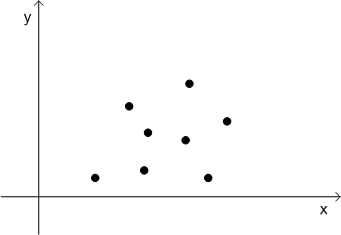
\includegraphics[scale=.3]{Original.eps}
\label{fig:concrete}
}
\subfigure[Intervals]
{
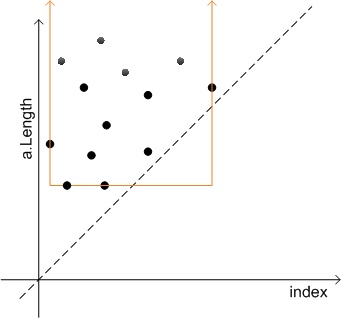
\includegraphics[scale=.3]{Intervals.eps}
\label{fig:intervals}
}
\subfigure[Octagons]
{
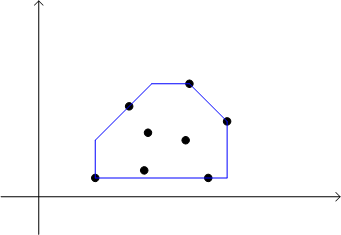
\includegraphics[scale=.3]{Octagons.eps}
\label{fig:octagons}
}
\subfigure[Pentagons]
{
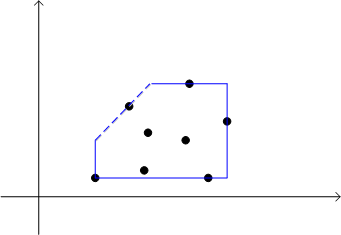
\includegraphics[scale=.3]{Pentagons.eps}
\label{fig:pentagons}
}
\caption{The concrete points, and some approximations depending on the numerical abstract domain}
\label{fig:example}
\end{figure*}

\section{Numerical Abstract Domains}
Abstract interpretation is a theory of approximations, \cite{CousotCousot77}.
It captures the intuition that semantics are more or less precise depending on the observation level.
The observation level is formalized by the notion of an abstract domain.
An abstract domain \adom{D} is a complete lattice \tupla{\el{E},\aless, \abot, \atp, \acup, \acap}, where \el{E} is the set of abstract elements, ordered according to relation $\aless$. 
The smallest abstract element is $\abot$, the largest is $\atp$. 
The join \acup, and the meet \acap,  are also defined.
When the abstract domain \adom{D} does not respect the ascending chain condition, then a widening operator \awidening{} must be used to enforce the termination of the analysis.
With a slight abuse of notation, sometimes we will confuse an  abstract domain \adom{D} with the set of its elements \el{E}.

An abstract domain \adom{D}, is related to a concrete domain \dom{C} by a monotonic concretization function, $\gamma \in \funzione{\adom{D}}{\dom{C}}$.
A \emph{numerical} abstract domain \adom{N} is an abstract domain
which approximates sets of numerical values, \eg, one such
concretization is  $\gamma \in \funzione{\adom{N}}{\parti{\Sigma}}$, where
$\Sigma = \funzione{\code{Vars}}{\mathbb{Z}}$ is an environment,
mapping variables to integers.

When designing numerical abstract domains, one wants to fine tune the
cost-precision ratio.  Consider the points in Fig.~\ref{fig:concrete}.
They represent the concrete values that two variables, \code{x} and \code{y},
can take at a given program point for \emph{all} possible
executions.  As there may be many such values or an unbounded number
of them, computing this set precisely is either too expensive or
infeasible. Abstract domains over-approximate such sets and thereby
make them tractable.

\subsubsection*{Intervals} 
A first abstraction of the points in Fig~\ref{fig:concrete} can be
made by retaining only the minimum and maximum values of variables \code{x} and \code{y}.
This is called interval abstraction. Graphically, it boils down to enveloping the concrete values with a rectangle, as depicted in Fig.~\ref{fig:intervals}.
The abstract domain of intervals is very cheap, as it requires
storing only two integers for each variable, and all the operations can be performed in linear time (w.r.t. the number of variables).
However, it is also quite imprecise, in particular because it cannot capture relations between variables.
For instance, in Fig.~\ref{fig:intervals} the fact that $\code{y} < \code{x}$ is lost.
 

\subsubsection*{Octagons}
A more precise abstraction is obtained by using the abstract domain of Octagons, \Octagons. 
\Octagons{} keeps relations of the form $\pm \code{x} \pm \code{y} \leq k$.
When applied to our concrete points, the octagon enveloping them is shown in Fig.~\ref{fig:octagons}.
\Octagons{} can capture relations between two variables---desirable
when analyzing array bounds---but its complexity is $\Order{n^2}$ in space and $\Order{n^3}$ in time.
The cubic complexity is a consequence of the closure algorithm used by all the domain operations.
Bagnara \emph{et al.} gave a precise bound for it in \cite{Bagnara05}. The standard closure operator on \Octagons{} performs $20 n^3 + 24  n^2$ coefficient operations, that can be reduced to $16n^3 + 4n^2 +4n$ with a smarter algorithm.

While having polynomial complexity, \Octagons{} unfortunately does not
scale if many variables are kept in the same octagon.
For this reason the technique of buckets has been independently introduced in  \cite{BlanchetCousotEtAl03} and \cite{Venet04}.
The intuition behind it is to create many octagons, each relating few variables, \eg,  no more than $4$.
The problem with this technique is how to choose the bucketing of
variables. Existing heuristics use the structure of the source program.

\subsubsection*{Pentagons}
The approximation of the concrete points with \Pentagons{} is given in Fig.~\ref{fig:pentagons}.
Elements of \Pentagons{} have the form of $\code{x} \in [a, b] \wedge \code{x} < \code{y}$, where $\code{x}$ and $\code{y}$ are variables and $a$ and $b$ belong to some underlying numerical set as $\mathbb{Z}$ or $\mathbb{Q}$.
A pentagon keeps lower and upper bounds for each variable, so it is as precise as intervals, but it also keeps strict inequalities among variables so that it enables a (limited) form of symbolic reasoning.
It is worth noting that the region of the plane that is delimited by a (two dimensional) pentagon may not be closed.
If fact, if the underlying numerical values are in $\mathbb{Q}$, then $\code{x} < \code{y}$ denotes an open surface of $\mathbb{Q}^2$, whereas if they are in $\mathbb{Z}$, then $\code{x} < \code{y}$ is equivalent to $\code{x} \leq \code{y} -1$, which is a closed region of $\mathbb{Z}^2$.

We found pentagons quite efficient in practice. 
The complexity is $\Order{n^2}$, both in time and space.
Furthermore, in our implementation we perform the expensive operation
(the closure) either lazily or in an incomplete (but sound) way, so
that the domain shows an almost linear behavior in practice.

\section{Interval Environments}
The elements of the abstract domain of intervals, \Intervals, are $\{ [i, s] \mid i,s \in \mathbb{Z} \cup \{-\infty, + \infty\} \}$.
The formal definition of the lattice operations on intervals is recalled in Tab.~\ref{tab:intervals}.
The order is the interval inclusion, the bottom  element is the empty interval (\ie, an interval where $s < i$), the largest element is the line $[-\infty, +\infty]$, the join and the meet are respectively the union and the intersection of intervals.
The widening preserves the bounds which are stable. 

The concretization function, $\gamma_\Intervals \in \funzione{\Intervals}{\parti{\mathbb{Z}}}$ is defined as $\gamma_\Intervals([i, s]) = \{ z \in \mathbb{Z} \mid i \leq z \leq s\}$.

\begin{table}[t]
\small
\begin{tabular}{rl}
Order:& $[a_1, b_1] \iless [a_2, b_2] \Longleftrightarrow a_1 \geq a_2 \wedge b_1 \leq b_2$ \\
Bottom:& $ [a, b] = \ibot \Longleftrightarrow a > b$ \\
Top:& $[a, b] = \itop \Longleftrightarrow a = -\infty \wedge b = +\infty$\\
Join:& $[a_1, b_1] \ijoin [a_2, b_2] = [\mathrm{min}(a_1, a_2), \mathrm{max}(b_1, b_2)]$ \\
Meet:& $[a_1, b_1] \imeet [a_2, b_2] = [\mathrm{max}(a_1, a_2), \mathrm{min}(b_1, b_2)]$ \\
Widening:& $[a_1, b_1] \iwidening [a_2, b_2] = [a_1 > a_2 ? a_2 : -\infty, b_1 < b_2 ? b_2 : +\infty]$ \\
\end{tabular}
\caption{Lattice operations over single intervals}
\label{tab:intervals}
\end{table}

The abstract domain of interval environments, \Boxes, is the functional lifting of \Intervals, \ie, $\Boxes =  \funzione{\Vars}{\Intervals}$.
The lattice operations are hence the functional extension of those in Tab.~\ref{tab:intervals}, as shown by Tab.~\ref{tab:boxes}.

The concretization of a box, $\gamma_\Boxes \in \funzione{\Boxes}{\parti{\Sigma}}$ is defined as $\gamma_\Boxes(f) = \{ \sigma \in \Sigma \mid \forall \code{x}. \code{x} \in f \Longrightarrow \sigma(\code{x}) \in \gamma_\Intervals(f(\code{x}))\}$.

The assignment and the guards in the interval environment are defined as usual in interval arithmetic.

\section{Strict upper bounds}
The abstract domain of strict upper bounds \SUB{} is a special case of the zone abstract domains, which keeps symbolic information in the form of $\code{x} < \code{y}$.
We represent elements of \SUB{} with maps $\code{x} \mapsto \{ \code{y}_1, \dots \code{y}_n \}$ with the meaning that \code{x} is strictly smaller than each of the $\code{y}_i$.
The formal definition of the lattice operations for \SUB{} is in Tab.~\ref{tab:sub}.

\begin{table}[h]
\small
\begin{tabular}{rl}
Order:& $ s_1 \sless s_2 \Longleftrightarrow \forall \code{x} \in s_2. s_1(\code{x}) \supseteq s_2(\code{x})$ \\
Bottom:& $ s = \sbot \Longleftrightarrow  \exists \code{x,y} \in s. \code{y} \in s(\code{x}) \wedge \code{x} \in s(\code{y})$ \\
Top:& $ s = \sTop \Longleftrightarrow \forall \code{x} \in s. s(\code{x}) = \emptyset$\\
Join:& $ s_1 \sjoin s_2 = \lambda \code{x}. s_1(\code{x}) \cap s_2(\code{x}) $ \\
Meet:& $ s_1 \smeet s_2 = \lambda \code{x}. s_1(\code{x}) \cup s_2(\code{x}) $  \\
Widening:&  $s_1 \swidening s_2 = \lambda \code{x}. s_1(\code{x}) \supseteq s_2(\code{x}) ? s_2(\code{x}) : \emptyset $
\end{tabular}
\caption{Lattice operations of strict upper bounds}
\label{tab:sub}
\end{table}
\hyphenation{pre-sent}
Roughly, the fewer constraints the less information is  present.
As a consequence, the order is given by the (pointwise) superset inclusion, the bottom environment is one which contains a contradiction $\code{x} < \code{y} \wedge \code{y} < \code{x}$ and the lack of information, \ie, the top element is represented by the empty set.
The join is (pointwise) set intersection: at a join point we want to keep those relations that hold on both (incoming) branches.
The meet is (pointwise) set union: relations that hold on either the left \emph{or} the right branch.
Finally, widening is defined in the usual way: we keep those
constraints that are stable in successive iterations (if the number of
variables is fixed, the join suffices).

The concretization function, $\gamma_\SUB \in \funzione{\SUB}{\parti{\Sigma}}$ is defined as $\gamma_\SUB(s) = \cap_{\code{x} \in s} \{ \sigma \in \Sigma \mid \code{y} \in s(\code{x}) \Longrightarrow \sigma(\code{x}) < \sigma(\code{y}) \}$.

\begin{table}
\small
\begin{tabular}{rl}
Order:& $ b_1 \bless b_2 \Longleftrightarrow \forall \code{x} \in b_1. b_1(\code{x}) \iless b_2(\code{x})$ \\
Bottom:& $ b = \bbot \Longleftrightarrow \exists \code{x} \in b. b(\code{x}) = \ibot$ \\
Top:& $ b = \btop \Longleftrightarrow \forall \code{x} \in b. b(\code{x}) = \itop$\\
Join:& $ b_1 \bjoin b_2 = \lambda \code{x}. b_1(\code{x}) \ijoin b_2(\code{x}) $ \\
Meet:& $ b_1 \bmeet b_2 = \lambda \code{x}. b_1(\code{x}) \imeet b_2(\code{x}) $  \\
Widening:&  $b_1 \bwidening b_2 = \lambda \code{x}. b_1(\code{x}) \iwidening b_2(\code{x}) $
\end{tabular}
\caption{Lattice operations of interval environments}
\label{tab:boxes}
\end{table}
 

\subsubsection*{The Need for Closure}

We deliberately skipped the discussion of the closure operation until now.
One may expect to endow the \SUB{} abstract domain with a
saturation rule for transitivity such as
\[
\frac{\code{y} \in s(\code{x}) \quad \code{z} \in s(\code{y})}{\code{z} \in s(\code{x})}
\]
and apply it to the abstract values prior to applying the join in
Tab.~\ref{tab:sub}, thereby inferring and retaining the maximum possible constraints.
However it turns out that the systematic application of the saturation
rule requires $\Order{n^3}$ operations, which voids the efficiency
advantage of \Pentagons.
In \Clousot, we chose to not perform the closure, and instead improved
the precision of individual transfer functions.
 They infer new relations $\code{x} < \code{y}$ and use a limited transitivity driven by the program under analysis. 
So, for instance:
\[
\begin{array}{rcl}
\sem{x := y - 1}(s) & = & s[\code{x} \mapsto \{ \code{y}\}] \\ 
\sem{x == y}(s) & = & s[\code{x}, \code{y} \mapsto s(\code{x}) \cup s(\code{y})] \\
\sem{x < y}(s) &=& s[\code{x} \mapsto s(\code{x}) \cup s(\code{y}) \cup \{ \code{y}\}] \\
\sem{x \leq y}(s) &=& s[\code{x} \mapsto s(\code{x}) \cup s(\code{y})]  
\end{array}
\]
because we know that i) if we subtract a positive constant from a
variable we obtain a result strictly smaller \footnote{In this paper
  we ignore overflows. However our abstract semantics of arithmetic
  expressions in \Clousot{} takes care of them.}, that ii) when we
compare two variables for equality they must satisfy the same
constraints, and that iii) for each $\code{z}$ such that $\code{y} < \code{z}$, if  $\code{x} < \code{y}$ or $\code{x} \leq \code{y}$ then $\code{x} < \code{z}$.

\section{Pentagons}
A first approach to combine the numerical properties captured by \Intervals, and the symbolic ones captured by \SUB{} is to consider the cartesian product  $\Intervals \times \SUB$.
Such an approach is equivalent to running the two analyses in parallel, without any exchange of information between the two domains.
A better solution is to perform the \emph{reduced} cartesian product $\Intervals \otimes \SUB$,~\cite{CousotCousot79}.
The elements of the reduced cartesian product satisfy the following relation
 \[
\forall \tupla{b, s} \in \Intervals \otimes \SUB. \gamma_{\Intervals \otimes \SUB}(\tupla{b, s}) \subseteq \gamma_{\Intervals}(b) \cap \gamma_{\SUB}(s) \,
\]
\ie, the analysis on the reduced lattice is more precise than the pairwise composition of the two analyses.
The \Pentagons{} abstract domain is an abstraction of the reduced product and is more precise than the cartesian product: 
\[
\Intervals \otimes \SUB \prec \Pentagons \prec \Intervals \times \SUB.
\]

The lattice operations are defined in Tab.~\ref{tab:pentagons}.
The functions $\mathrm{sup}$ and $\mathrm{inf}$ are defined as  $\mathrm{inf}([a,b]) = a$ and $\mathrm{sup}([a,b]) = b$.

The order on pentagons is a refined version of the pairwise order: a pentagon $\tupla{b_1, s_1}$ is smaller than a pentagon $\tupla{b_2, s_2}$ iff the interval environment $b_1$ is included in $b_2$ and for all the symbolic constraints $\code{x} < \code{y}$ in $s_2$, either $\code{x} < \code{y}$ is an explicit constraint in $s_1$ or it is implied by the interval environment $b_1$, \ie, the numerical upper bound for \code{x} is strictly smaller than the numerical lower bound for \code{y}.

A pentagon is bottom if either its numerical component \emph{or} the symbolic component are.
A pentagon is top if both the numerical component \emph{and} the symbolic component are.

For the numerical part, the join operator pushes the join to the underlying \Intervals{} abstract domain, and for the symbolic part, it keeps the constraints which are either explicit in the two operators \emph{or} which are explicit in one operator, and implied by the numerical domain in the other component. 
We will further discuss the join, cardinal for the scalability and the precision of the analysis below.

The meet and the widening operators simply delegate the meet and the widening to the underlying abstract domains.
Note that we do not perform any closure before widening in order to
avoid well known convergence problems arising from the combination of widenings and closure operations~\cite{Mine01-2}.

\begin{table}
\small
\begin{tabular}{rl}
Order:& $\tupla{b_1, s_1} \pless \tupla{b_2, s_2}   \Longleftrightarrow  b_1 \bless b_2 $ \\
& $ \quad \wedge (\forall \code{x} \in s_2 \forall\code{y} \in s_2(\code{x}).$ \\
& $\quad \quad \quad  \code{y} \in s_1(\code{x}) \vee\ \mathrm{sup}(b_1(\code{x})) < \mathrm{inf}(b_1(\code{y}))) $ \\
Bottom:& $\tupla{b, s}  = \pbot \Longleftrightarrow b = \bbot \vee  s = \sbot $ \\
Top:& $ \tupla{b, s} = \ptop \Longleftrightarrow b = \btop \wedge s = \sTop $\\
Join:& $\tupla{b_1, s_1}  \pjoin  \tupla{b_2, s_2}  = $ \\
& $\quad \mathrm{let}\ b^\sqcup = b_1 \bjoin b_2$ \\
& $\quad \mathrm{let}\ s^\sqcup = \lambda \code{x}.  s'(\code{x}) \cup s''(\code{x}) \cup s'''(\code{x})$ \\
& $\quad \quad \mathrm{where}\ s' = \lambda \code{x}. s_1(\code{x}) \cap s_2(\code{x})$ \\
& $\quad \phantom{\lambda \code{x}.} \mathrm{and}\ s'' = \lambda \code{x}. \{\code{y} \in s_1(\code{x}) \mid \mathrm{sup}(b_2(\code{x})) < \mathrm{inf}(b_2(\code{y})) \}$ \\
& $\quad  \phantom{\lambda \code{x}.} \mathrm{and}\ s''' =  \lambda \code{x}. \{\code{y} \in s_2(\code{x}) \mid \mathrm{sup}(b_1(\code{x})) < \mathrm{inf}(b_1(\code{y})) \}$ \\
& $\quad \mathrm{in}\ \tupla{ b^\sqcup, s^\sqcup}$ \\
Meet:& $ \tupla{b_1, s_1}  \pmeet  \tupla{b_2, s_2}  = \tupla{b_1 \bmeet b_2, s_1 \smeet s_2} $  \\
Widening:&  $ \tupla{b_1, s_1}  \pwidening \tupla{b_2, s_2}  = \tupla{b_1 \bwidening b_2, s_1 \swidening s_2}$
\end{tabular}
\caption{The lattice operations over pentagons}
\label{tab:pentagons}
\end{table} 


\subsubsection*{Cost and Precision of the Join}
One may ask why we defined the join over \Pentagons{} as in Tab.~\ref{tab:pentagons}.
In particular, a more natural definition may be to first close the two operands, by deriving all the symbolic and numerical constraints, and then perform the join.
This is for instance how the standard join of \Octagons{} works.
More formally one may want to have a closure for a pentagon $\tupla{b,
  s}$ defined by:
\[
\begin{array}{l}
b^* = \bigsqcap_{\code{x} < \code{y} \in s} \semantica{}{\code{x} < \code{y}}(b) \\
s^* = \lambda \code{x}. s(\code{x}) \cup \{ \code{y} \in b\mid \code{x} \neq \code{y} \Longrightarrow \mathrm{sup}(b^*(\code{x})) < \mathrm{inf}(b^*(\code{y}))\} 
\end{array}
\]
The closure first refines  the interval environment by assuming all the strict inequalities of the \SUB{} domain.
Then, it closes the element of the \SUB{} domain by adding all the strict inequalities implied by the numerical part of the abstract domain.

As a consequence, the closure-based join $\pjoin^*$ can be defined as 
\[
\tupla{b_1, s_1} \pjoin^* \tupla{b_2, s_2} = \tupla{b_1^* \bjoin b_2^*, s_1^* \sjoin s_2^* } 
\]
The complexity of $\pjoin^*$ is $\Omega(n^2)$, as for getting  $s^*$  we need to consider all the pairs of intervals in $b^*$.

Performing a quadratic operation at each join point imposes a serious
slowdown of the analysis.
In our experience, when used for \code{mscorlib.dll}, we got that the running time of the analyzer went up to more than $45$ minutes. 

As a consequence we defined a safe approximation of the join as in Tab.~\ref{tab:pentagons}.
The idea behind $\pjoin$ is to avoid materializing new symbolic constraints, but just to keep those which are present in one of the two operators, and implied by the numerical part of the other operand.
If needed, some implied relations may be recovered later (hence lazily),
after the join point. The next example illustrates this on an
assertion following a join point.

\textit{Example.}
Let us consider the code in Fig.~\ref{fig:ex1a}, to be analyzed with some initial pentagon $\tupla{b, s}$ which does not mention \code{x} and \code{y}.
Using $\pjoin^*$, one gets the post-state 
\[ 
p_1 = \tupla{b[\code{x} \mapsto [-2, 0], \allowbreak \code{y} \mapsto [1, 3]], \allowbreak s[\code{x} \mapsto \{ \code{y} \} ]}.
\]
With $\pjoin$ the result is 
\[
p_2 = \tupla{b[\code{x} \mapsto [-2, 0], \allowbreak \code{y} \mapsto [1,3]], \allowbreak s]}.
\]
Suppose that we'd like to discharge $\code{assert\ x < y}$ following the conditional.
The first pentagon, $p_1$ already contains the constraint $\code{x} <
\code{y}$, thus proving the assertion is as complex as a simple  table lookup.
On the other hand, the symbolic part of $p_2$ does not contain the
explicit constraint $\code{x} < \code{y}$, but it is implied by the
numerical part. Proving the assertion with $p_2$ requires two table lookups and an integer comparison. 
\qed
 
One may argue that  $\pjoin$ is just a lazy version of $\pjoin^*$. 
However it turns out that the abstraction is strict, in that there are cases where $\pjoin$ introduces a loss of information that cannot be recovered later, as shown by the next example.

\textit{Example.}
Let us consider the code in Fig.~\ref{fig:ex1b}, to be analyzed with some initial pentagon $\tupla{b, s}$, which does not mention \code{x} and \code{y}.
Using the closure-based join, $\pjoin^*$ one obtains the pentagon
\[ 
p_3 = \tupla{b[\code{x} \mapsto [-2, 0], \allowbreak \code{y} \mapsto [0, 3]], \allowbreak s[\code{x} \mapsto \{ \code{y} \} ]}.
\]
which implies that $\code{x}$ and $\code{y}$ cannot be equal to $0$ at the same time.
On the other hand, $\pjoin$ returns
\[
p_4 = \tupla{b[\code{x} \mapsto [-2, 0], \allowbreak \code{y} \mapsto [0,3]], \allowbreak s]}.
\] 
which does not exclude the case when $\code{x} = \code{y} = 0$.
As a consequence, $\code{assert}\ \code{x} + \code{y} \neq 0$ cannot be proved using $p_4$, whereas it can be with $p_3$.
\qed

Even if the previous example shows that there may be some loss of
precision induced by using \pjoin, we found it negligible in practice
(see Sect.~\ref{sec:experiments}).
We also tried a hybrid solution, where we fixed some
$\overline{n}$. If the cardinality of the abstract elements to join
was $n<\overline{n}$, then the we used $\pjoin^*$, otherwise we used
$\pjoin$. However, we did not find any values for $\overline{n}$ with
a better cost-precision trade-off.

\begin{figure}
\centering
\subfigure[Non-strict abstraction]
{
\begin{tabular}{l}
  \code{if\ (...)} \\
  \quad\code{ x = 0;\ y = 3;} \\
  \code{else}  \\
  \quad \code{x = -2;\ y = 1};\hspace*{10mm}
\end{tabular}
\label{fig:ex1a}
}
\subfigure[Strict abstraction]
{
\begin{tabular}{l}
  \code{if\ (...)} \\
  \quad\code{ x = 0;\ y = 3;} \\
  \code{else}  \\
  \quad \code{x = -2;\ y = 0};
\end{tabular}
\label{fig:ex1b}
}
\caption{Difference in precision between $\pjoin^*$ and $\pjoin$}
\end{figure}


\begin{table*}
\centering
\small
\begin{tabular}{@{}r r |r r r| r r r | r r r| r r r@{}}
         &  Bounds              & \multicolumn{3}{c|}{\Intervals} & \multicolumn{3}{c|}{$\Intervals \times \SUB$}      & \multicolumn{3}{c|}{\Pentagons{} $\pjoin$} &  \multicolumn{3}{c}{\Pentagons{} $\pjoin^*$}  \\
Assembly & checked & Valid & \% & Time & Valid & \% & Time &
Valid & \% & Time & Valid & \% & Time   \vspace{3pt}  \\

\hline
\code{mscorlib.dll}      & 17 052 & 12 416 & 72.79 & 5:08 & 14 059 & 82.42 & 7:03 & 14 162 & 83.02 & 7:25 & 14 162 & 83.02 & 61:39 \\
\code{System.dll}        & 11 609 &  9 298 & 80.09 & 3:38 &  9 979 & 85.95 & 4:56 &  9 993 & 86.07 & 5:10 &      - &     - &     - \\
\code{System.Web.dll}    & 14 202 & 12 313 & 86.69 & 3:54 & 12 952 & 91.19 & 5:39 & 12 964 & 91.28 & 5:49 & 12 964 & 91.28 & 18:55 \\
\code{System.Design.dll} & 10 072 &  8 854 & 87.90 & 3:52 &  9 562 & 94.93 & 5:01 &  9 586 & 95.17 & 5:17 &  9 610 & 95.41 & 43:18 \\
\hline
Average                  &        &        & 80.99 &      &        & 87.92 &      &        & 88.22 &      &        &     - &       \\
\end{tabular}
\caption{The experimental results of the analyzer with different abstract domains}
\label{tab:results}
\end{table*}

\subsubsection*{Transfer Functions}
Analysis precision also heavily depends on the precision of the transfer functions.
Using \Pentagons{} we can refine the transfer functions for some MSIL instructions  which have a non-trivial behavior depending on the operators.

Let us illustrate this situation using the $\mathtt{rem}$ instruction of MSIL.
Intuitively, $\mathtt{rem}\ \code{u\ d} $ computes the reminder of the division $\code{u / d}$.
The precise handling of the remainder is important as many expressions
used to access arrays in \code{mscorlib.dll} include the remainder operation.
According to the definition of \code{rem} in Part. III, Sect. 3.55 of
\cite{ECMA-CLI}, the sign of the result is the sign of $\code{u}$ and
$0 \leq | \code{rem \ u \ d} | < | \code{d} |$ holds. 
Therefore in order to derive the constraint $\code{rem \ u \ d} < \code{d}$ one
must know that $\code{d} \geq 0$.  

The transfer function for \code{rem} in \Intervals{} can infer useful
upper bounds whenever \code{d} is finite, but it infers unhelpful
bounds when \code{d} is infinite.

The transfer function for \code{rem} in \SUB{} cannot infer lower
bounds, and worse, no upper bounds, for it cannot
determine the sign of \code{d}.

The transfer function for \code{rem} in \Pentagons{} has the necessary
information. It uses \Intervals{} to determine if \code{d} is
non-negative in the pre-state,
then constrains the result using \SUB{}, modeling the assignment more precisely.
\begin{multline*}
\semantica{}{x := rem\ u\ d}(\tupla{b, s}) = \\ 
\tupla{\semantica{}{x := rem\ u\ d}(b), s[\code{x} \mapsto (\mathrm{inf}(b(\code{d})) \geq 0) ? \{ \code{d} \}: \emptyset  }
\end{multline*}

\section{Experiments}\label{sec:experiments}
We have implemented the abstract domain \Pentagons{} in our analyzer
for .NET assemblies, \Clousot. Prior to the array bound analysis,
\Clousot{} performs heap abstraction and expression analysis.
For arrays, \Clousot{} tries to validate that (i) the expression for a
\code{newarr} instruction is non-negative, and (ii) the
index for the 
\code{ldelem}, \code{stelem}, and \code{ldelema} instructions is greater than or
equal to zero and strictly smaller than the length of the array.
All experiments were conducted on a Centrino 2 duo processor at 2.16
GHz, with 4 GB of RAM, running Windows Vista. 

Tab.~\ref{tab:results} summarizes the results of running the analysis
on a subset of the .NET framework assemblies. 
 The analyzed assemblies
are taken from the directory \code{\%WINDIR\% \backslash \allowbreak
Microsoft\allowbreak \backslash} \code{Framework\backslash\allowbreak
  v\allowbreak2.0.\allowbreak50727} of 
our laptop without modification or preprocessing.

We ran the analysis with four different domains, shown in the
different columns: intervals alone, the cartesian product
\Intervals$\times$\SUB, \Pentagons{} without constraint closure, and
finally \Pentagons{} with constraint closure. 

The table shows that combining \Intervals{} with symbolic upper bounds
validates on average almost 7\% more array accesses than \Intervals{}
alone for only a modest extra cost. \Pentagons{} without closure
validate an extra 0.3\% of accesses at little extra cost, whereas
\Pentagons{} with closure produces almost no extra precision but the
analysis time blows up. The time for the missing run was in excess of
90 minutes. Overall, the results show that with \Pentagons{}, \Clousot{} is able to
validate on average 88.2\% of all array accesses in under 7
minutes for the analyzed .NET assemblies.

As for the memory footprint, the analyzer never exceeded 300 Mbytes of RAM.
\smallskip

\section{Conclusions}
We presented a new numerical abstract domain, \Pentagons.  We
described its lattice operations, discussed its complexity and
presented an optimized algorithm for the join operator which runs in
(almost) linear time (instead of quadratic).

This abstract domain sits, as precision and cost are concerned, in
between the abstract domains of intervals and octagons.

We used \Pentagons{} to validate on average over 88\% of array
accesses in four major .NET assemblies in a couple of minutes. We plan
to discharge the remaining unproven accesses by using more
precise, yet expensive domains on demand.

\textit{Acknowledgments.} We would like to thank the Anindya Banerjee, Pietro Ferrara and the anonymous referees.

\begin{thebibliography}{10}
\small

\bibitem{Bagnara05}
R.~Bagnara, P.~M. Hill, E{.}Mazzi, and E.~Zaffanella.
\newblock Widening operators for weakly-relational numeric abstractions.
\newblock In {\em SAS'05}. Springer-Verlag, Sept. 2005.

\bibitem{BlanchetCousotEtAl03}
B.~Blanchet, P.~Cousot, R.~Cousot, J.~Feret, L.~Mauborgne, A.~Min\'e,
  D.~Monniaux, and X.~Rival.
\newblock A static analyzer for large safety-critical software.
\newblock In {\em PLDI'03}. ACM Press, June 2003.

\bibitem{Cousot03}
P.~Cousot.
\newblock Verification by abstract interpretation.
\newblock In {\em Verification: Theory and Practice}. Springer-Verlag, 2003.

\bibitem{CousotCousot77}
P.~Cousot and R.~Cousot.
\newblock Abstract interpretation: a unified lattice model for static analysis
  of programs by construction or approximation of fixpoints.
\newblock In {\em POPL'77}. ACM press, Jan. 1977.

\bibitem{CousotCousot79}
P.~Cousot and R.~Cousot.
\newblock Systematic design of program analysis frameworks.
\newblock In {\em POPL '79}, pages 269--282. ACM Press, Jan. 1979.

\bibitem{CousotHalbwachs78}
P.~Cousot and N.~Halbwachs.
\newblock Automatic discovery of linear restraints among variables of a
  program.
\newblock In {\em POPL '78}. ACM Press, Jan. 1978.

\bibitem{ECMA-CLI}
ECMA.
\newblock {S}tandard {ECMA-335}, {C}ommon {L}anguage {I}nfrastructure ({CLI}).
\newblock
  http://www.ecma-international.org/\-publications/\-standards/\-ecma-335.htm,
  Ecma International, 2006.

\bibitem{Logozzo07}
F.~Logozzo.
\newblock Cibai: An abstract interpretation-based static analyzer for modular
  analysis and verification of {Java} classes.
\newblock In {\em VMCAI'07}. Springer-Verlag, Jan. 2007.

\bibitem{Mine01-2}
A.~Min\'e.
\newblock The octagon abstract domain.
\newblock In {\em WCRE 2001}. IEEE Computer Society, Oct. 2001.

\bibitem{Navas07}
J.~Navas, E.~Mera, P.~L{\'o}pez-Garc\'{\i}a, and M.~V. Hermenegildo.
\newblock User-definable resource bounds analysis for logic programs.
\newblock In {\em ICLP'07}. Springer-Verlag, Sept. 2007.

\bibitem{SimonKing02}
A.~Simon, A.~King, and J.~M. Howe.
\newblock Two variables per linear inequality as an abstract domain.
\newblock In {\em LOPSTR'02}. Springer-Verlag, 2002.

\bibitem{Venet02}
A.~Venet.
\newblock Nonuniform alias analysis of recursive data structures and arrays.
\newblock In {\em SAS'02}. Springer-Verlag, Sept. 2002.

\bibitem{Venet04}
A.~Venet and G.~P. Brat.
\newblock Precise and efficient static array bound checking for large embedded
  c programs.
\newblock In {\em PLDI'04}. ACM Press, July 2004.

\end{thebibliography}

%\small
%\bibliographystyle{abbrv}
%\bibliography{bib} 

\end{document}
